This is a brief chapter that might provide a sigh of relief. So many of the parameters we have tweaked so far, sometimes laboriously, can be altered in one go with \code{plt.style.use}. Try out the \link{https://matplotlib.org/stable/gallery/style_sheets/style_sheets_reference.html\#sphx-glr-gallery-style-sheets-style-sheets-reference-py}{many style sheets already available}.\footnote{https://matplotlib.org/stable/gallery/style\_sheets/style\_sheets\_reference.html\#sphx-glr-gallery-style-sheets-style-sheets-reference-py} You may also define your own or simply change certain parameters directly in your code to apply that styling for your entire session. 

\section{rcParams}

Change the matplotlib parameters directly by updating the dictionary-like variable \code{mpl.rcParams}. A full list of the available parameters can be found in the  \link{https://matplotlib.org/stable/api/matplotlib_configuration_api.html\#matplotlib.rcParams}{documentation} or you may simply print \code{mpl.rcParams} to inspect it directly. Note the above line is \code{mpl.rcParams} and not \code{plt.rcParams}, because we are not working within the pyplot submodule. Accordingly, you'll have to run \code{import matplotlib as mpl} first. Because this is like a Python dictionary, you can adjust the settings by simply updating the dictionary value, \code{mpl.rcParams['axes.grid'] = True} for example. 

Working with \code{rcParams}, directly or through a custom style sheet, provides value that compounds as you add more and more plots to your code.  Consider the two programs below. Without \code{rcParams}, we update each plot.

\begin{lstlisting}[language = Python]
x = np.linspace(0,1,2)

fig, ax = plt.figure(), plt.axes()
ax.plot(x, x)
ax.grid(True)
ax.spines['top'].set_visible(False)
ax.spines['right'].set_visible(False)
plt.show()

fig, ax = plt.figure(), plt.axes()
ax.plot(x, 1 - x)
ax.grid(True)
ax.spines['top'].set_visible(False)
ax.spines['right'].set_visible(False)
plt.show()
\end{lstlisting}

\vspace{-0.3cm}
Now let's update \code{rcParams} just once for a standard style.

\vspace{-0.3cm}
\begin{lstlisting}[language = Python]
# Use rcParams
mpl.rcParams['axes.grid'] = True
mpl.rcParams['axes.spines.top'] = False
mpl.rcParams['axes.spines.right'] = False

x = np.linspace(0,1,2)

plt.plot(x,x)
plt.show()

plt.plot(x, 1-x)
plt.show()
\end{lstlisting}
\vspace{-0.5cm}
\begin{center}
    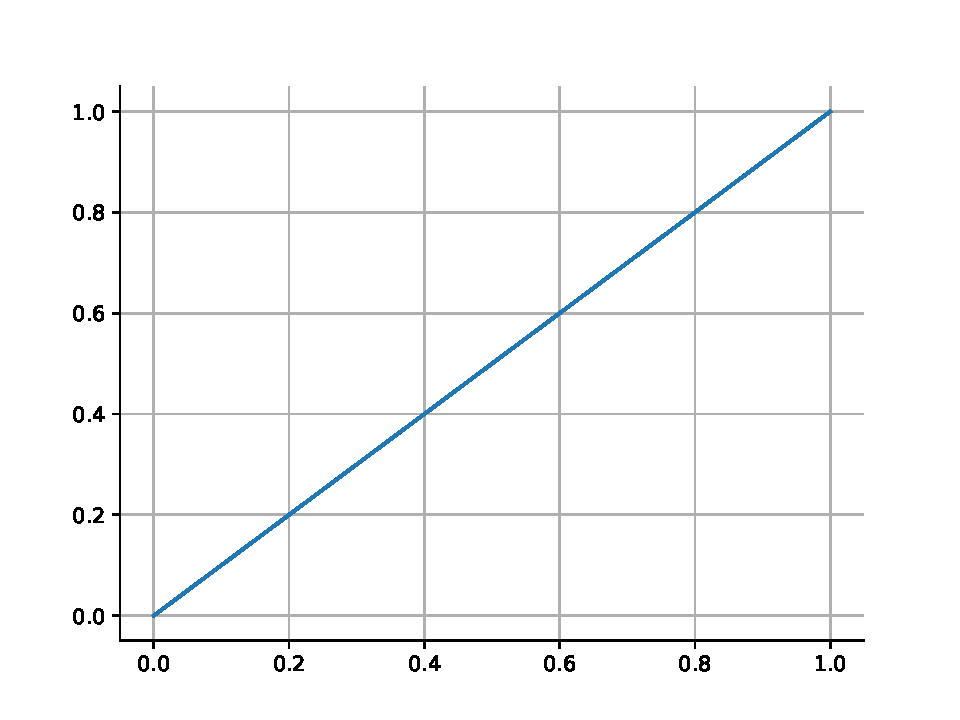
\includegraphics[width = .7\textwidth]{Images/style1.pdf}
    
    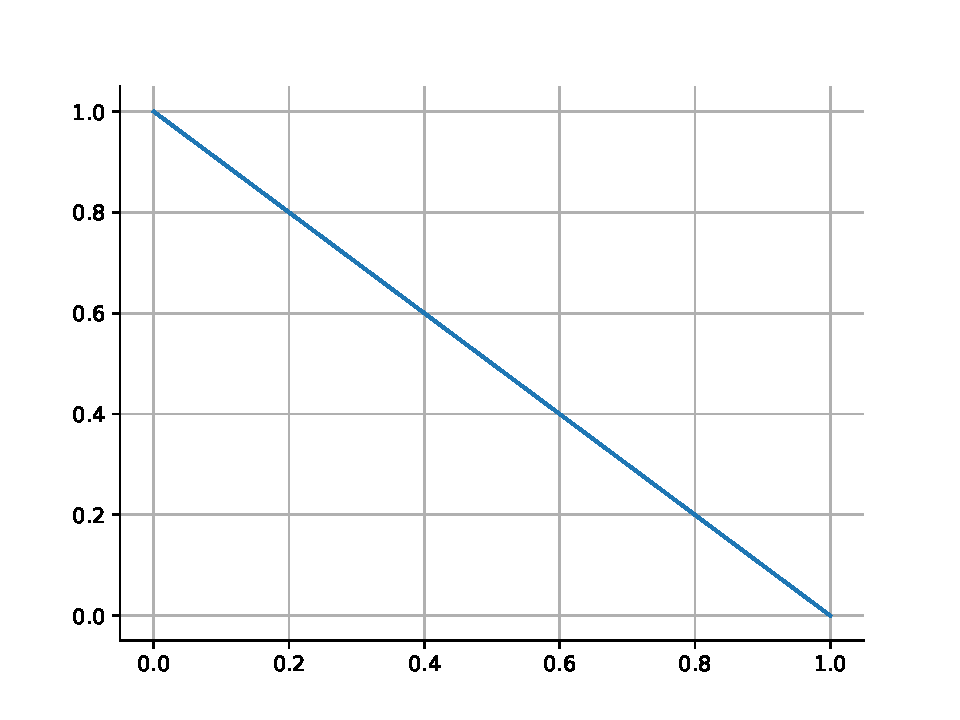
\includegraphics[width = .7\textwidth]{Images/style2.pdf}
\end{center}


This is a significant step, nearing us to a dramatic close of Part \ref{part:prose}. In the second program, we not only save on redundant code, we also revert back to pyplot functions. The object-oriented approach was useful in offering greater customization. But, at least in this case, that's a ladder we can kick away now that we've climbed it to the top.  

\section{Defining Your Own Style}

Once you understand rcParams, you can define your own style for repeated use. \cite{schwabish2021better} counsels organizations to adopt a data visualization style guide. Practically, that also means matplotlib-using organizations should choose or create a standard matplotlib style. 

To define your own style, create a file with the \texttt{.mplstyle} extension, specifying a value for the various rcParams you wish to customize. Note that a colon separates the key and the default like in a dictionary, but that we do not separate key-value pairs by commas and each pair is on a separate line. Further, none of these values are formatted as strings, even though you would, for example, use a string \code{'Times'} when updating the font from rcParams dictionary. You only need to specify values you wish to change relative to the default.

\begin{lstlisting}[caption = {[tiny\_style.mplstyle]}] %skip
axes.spines.left : True
axes.spines.right : False
axes.spines.bottom : True
axes.spines.top : False
xtick.labelsize : large
font.family : Times
\end{lstlisting}

After saving the above as a file \texttt{tiny\_style.mplstyle} and placing it in the working directory, we can use our custom style with the program below. Note the colormap, among many other things, has not changed relative to the default because we did not alter that in the style file. 

\begin{lstlisting}[language = Python]
plt.style.use('tiny_style.mplstyle')

fig, ax = plt.figure(), plt.axes()
x = np.linspace(0,2*np.pi,100)
plt.plot(x, np.sin(x))
plt.plot(x, np.cos(x))
plt.title('Hello')

# Inspect the updated rcParams
print(mpl.rcParams)
\end{lstlisting}

\begin{center}
    \includegraphics[width = .7\textwidth]{proseplots/customStyle.png}
\end{center}

You can also just save direct modifications to the rcParams dictionary and run that before plotting. 

\begin{lstlisting}[language = Python,
caption = {[style\_changes.py]}]
import matplotlib as mpl
mpl.rcParams['axes.spines.left'] = True
mpl.rcParams['axes.spines.right'] = False
mpl.rcParams['axes.spines.bottom'] = True
mpl.rcParams['axes.spines.top'] = False
mpl.rcParams['axes.titlesize'] = 25
mpl.rcParams['xtick.labelsize'] = 'large'
mpl.rcParams['font.family'] = 'Times'
\end{lstlisting}

Then add this code to ahead of creating your plot. I saved the above as \texttt{style\_changes.py} and below I use the Jupyter \code{\%run} magic command to run \texttt{style\_changes.py} without having to copy and paste. 
\begin{lstlisting}[language = Python]
# uncomment to return to default style if still using tiny_style
#plt.style.use('default')
%run style_changes.py

x = np.linspace(0,2*np.pi,100)
plt.plot(x, np.sin(x))
plt.plot(x, np.cos(x))
plt.title('Hello')
\end{lstlisting}

The result is the same plot. 

\begin{center}
    \includegraphics[width = .7\textwidth]{proseplots/LongRouteStyle.png}
\end{center}

\subsection{Temporary Configurations}

%with plt.style.context(changes):

With some creativity, you can also avoid modifying rcParams by defining a function or writing a Python file that makes certain standardized plot modifications and then run that after you've created your figure and axes objects, using the IPython \code{\%run} magic command. 

We save the following as \texttt{spine\_mod.py} and then use it below to modify a plot. 
% double check me here


%%% can make good for subplots with 
%https://stackoverflow.com/questions/24104990/how-to-get-a-list-of-axes-for-a-figure-in-pyplot
% ax_list = fig.axes
\begin{lstlisting}[language = Python,caption = {[spine\_mod.py]}]
import matplotlib.pyplot as plt 

plt.gca().spines['left'].set_position('zero')
plt.gca().spines['bottom'].set_position('zero')

plt.gca().spines['top'].set_visible(False)
plt.gca().spines['right'].set_visible(False)
\end{lstlisting}


\begin{lstlisting}[language = Python]
x = np.linspace(0,2*np.pi,100)
plt.plot(x, np.sin(x))
plt.plot(x, np.cos(x))
plt.title('Spine Mods')

%run spine_mod.py
\end{lstlisting}

\begin{center}
    \includegraphics[width = .7\textwidth]{proseplots/SpineMod.pdf}
\end{center}

In the plot program, we use pyplot functions instead of using the OOP approach. Note that even if we created an \code{ax} variable, we must still use \code{plt.gca()} instead of \code{ax} in the file, because there is no \code{ax} to reference in \texttt{spine\_mod.py}\footnote{Variables outside the file are not in a shared \emph{scope} because \code{\%run} creates a new \emph{namespace} for variables inside the file)}. We can instead use \code{\%run -i} to let the file access our global variables. Also, \code{\%run -i} eliminates the need to import matplotlib again---we could delete the import statement from \texttt{spine\_mod.py} and use \code{\%run -i spine_mod.py}. 

We save the following file as \texttt{spine\_mod2.py} and can create the same plot with the program further below. 

\begin{lstlisting}[language = Python,caption = {[spine\_mod2.py]}]
ax.spines['left'].set_position('zero')
ax.spines['bottom'].set_position('zero')
ax.spines['top'].set_visible(False)
ax.spines['right'].set_visible(False)
\end{lstlisting}

\begin{lstlisting}[language = Python]
x = np.linspace(0,2*np.pi,100)
fig, ax = plt.figure(), plt.axes()
ax.plot(x, np.sin(x))
ax.plot(x, np.cos(x))
ax.set_title('Spine Mods')
%run -i spine_mod2.py
\end{lstlisting}

A further complication arises if our figure contains multiple subplots. In this case, we can access all the axes objects as an attribute of the figure object. 

% double check

\begin{lstlisting}[language = Python,caption = {[spine\_mod3.py]}]
for ax in fig.axes:
    ax.spines['left'].set_position('zero')
    ax.spines['bottom'].set_position('zero')
    ax.spines['top'].set_visible(False)
    ax.spines['right'].set_visible(False)
\end{lstlisting}



%See \link{https://matplotlib.org/stable/tutorials/introductory/customizing.html\#defining-your-own-style}{the documentation} for further details.

\section{A Final Prose Example}

In this section, we'll integrate much of what we've learned so far to create a line chart that, though simple, is far from the default. We'll imitate a chart from the New York Times article, \emph{The Pandemic Changed How We Spent Our Time}, by Ben Casselman and Ella Koeze. Below is the original. 

\begin{center}
    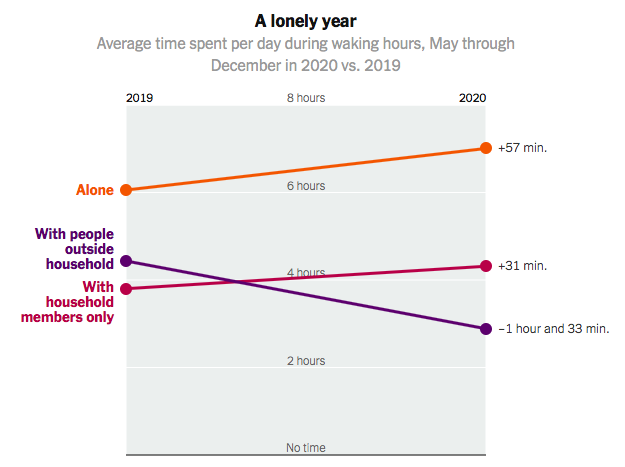
\includegraphics[width = .8\textwidth]{Images/nytATUS.png}
\end{center}

Imitating this graphic will take a lot of code, as demonstrated in Section \ref{subsec:firstgo}. In Section \ref{subsec:rrr}, we invest in reconfiguring the style and creating functions that  help reduce the tedium that would otherwise be required to make several plots of this style. 

\subsection{A First Go}\label{subsec:firstgo}

The program below would be even longer if not for the use of dictionaries like \code{plot_style}, which pairs pairs keyword arguments and specific values for the \code{plot()} method. This can be passed to \code{plot()} after being unpacked with the \code{**} operator. 

\begin{lstlisting}[language = Python]

fig = plt.figure(figsize = (7,6.5)) 
ax = plt.axes(facecolor = (.94, .94, .96))

## Add data and annotations
plot_style = dict(marker = 'o', 
        clip_on = False, # don't clip markers at axes boundary
        linewidth = 3,
        markersize = 8)
right_text_style = dict(ha = 'left', fontsize = 11, 
                      fontname = 'Helvetica',
                      color = (.3,.3,.3),
                      va = 'center')
left_text_style = dict(ha = 'right',
                      fontsize = 12,
                      fontweight = 'bold',
                      fontname = 'Helvetica')
x_vals = [2019,2020]
# alone
col = 'orange'
ax.plot(x_vals, [6,7], 
        color = col,  
        **plot_style)
ax.text(2019 - .02, 6, 'Alone', 
        color = col, 
        va = 'center',
        **left_text_style)
ax.text(2020.03, 7, '+57 min.', 
        **right_text_style)

# within household
col = 'purple'
ax.plot(x_vals, [4.3,2.7], 
        color = col,  
        **plot_style)
ax.text(2019 - .02, 4.2, 'With people\noutside\nhousehold', 
        color = col, 
        va = 'bottom',
        **left_text_style)
ax.text(2020.03, 2.7, '-1 hour and 33 min.', 
        **right_text_style)

# outside household
col = 'darkred'
ax.plot(x_vals, [3.9,4.4], color = col,  
        **plot_style)
ax.text(2019 - .02, 4, 'With\nhousehold\nmembers only', color = col, 
        va = 'top',
       **left_text_style)

ax.text(2020.03, 4.4, '+31 min.',
        **right_text_style)


# Label Gridlines
text_style = dict(color = (.3,.3,.3), 
                 va = 'bottom',
                 ha = 'center',
                 fontname = 'Helvetica',
                 fontsize = 11)  

ax.text(2019.5, 0.01, "No Time", **text_style)
for y in [2,4,6,8]:
    ax.text(2019.5, y+.04, "{} hours".format(y),
            **text_style)

# Label 2020/2021 for x-axis
year_text_style = dict(color = (.3,.3,.3), 
                 va = 'bottom',
                 fontname = 'Helvetica',
                 fontsize = 12)  
ax.text(2019, 8.05, '2019', 
                ha = 'left', **year_text_style)
ax.text(2020, 8.05, '2020',
                ha = 'right', **year_text_style)

# set main title
ax.set_title("A lonely year", pad = 55, fontweight = 'bold', 
             fontname = 'Helvetica',
            fontsize = 18)

# set subtitle
s = 'Average time spent per day during waking hours, May through\nDecember in 2020 vs. 2019'
ax.text(2019.5, 8.5, s, **text_style)

# x axis
ax.set_xticks([])
ax.set_xlim(2019,2020)

# y axis
ax.yaxis.grid(True, color = 'white')
ax.set_yticks([0,2,4,6,8])
ax.set_yticklabels([])
ax.set_ylim([-.02,8])
ax.yaxis.set_tick_params(length = 0, grid_linewidth = 2)

# spines
for i in ['top','left','right']:
    ax.spines[i].set_visible(False)
ax.spines['bottom'].set_color('darkgray')
ax.spines['bottom'].set_linewidth(2)
\end{lstlisting}


\begin{center}
    \includegraphics[width = .9\textwidth]{proseplots/NYTreplica2.png}
\end{center}

\subsection{Reconfigured, Refactored, and Reusable}\label{subsec:rrr}

\begin{lstlisting}[language = Python]
style_changes = {'axes.linewidth': 2,
 'axes.facecolor': (.94, .94, .96),
 'axes.grid.axis': 'y',
 'axes.grid': True,
 'grid.color': 'white',
 'grid.linewidth': 2,
 'axes.spines.bottom': True,
 'axes.spines.top': False,
 'axes.spines.left': False,
 'axes.spines.right': False,
 'axes.edgecolor': 'darkgray',
 'xtick.bottom': False,
 'xtick.top': False,
 'ytick.left': False,
 'xtick.labeltop':True,
 'xtick.labelbottom':False,
 'ytick.labelleft':False,
 'xtick.color': (.3,.3,.3),
 'text.color': (.3,.3,.3),
 'font.size': 12,
 'lines.marker': 'o',
 'lines.markersize': 8,
 'lines.linewidth': 3,
 'axes.titlesize': 18,
 'axes.titleweight': 'bold', 
 'axes.formatter.useoffset': False # prevent scientific notation
          }
\end{lstlisting}


\begin{lstlisting}
def title_and_subtitle(title, subtitle = '', pad = 0.01, fig = None, ax = None):
    """Add a centered title and subtitle to a plot."""
    if ax == None:
        ax = plt.gca()
    if fig == None:
        fig = plt.gcf()
    
    fig.canvas.draw()
    
    top_of_figure = 1 # axes coords
    # update if there are xticks on the top 
    top_of_ticklabels = ax.get_xticklabels()[0].get_window_extent().transformed(ax.transAxes.inverted()).y1
    top_of_figure = max([top_of_ticklabels,top_of_figure])
        
    # Add subtitle
    if subtitle:
        subt = ax.text(0.5, top_of_figure + pad, subtitle, 
               ha = 'center',
               va = 'bottom',
               size = '11',
               fontname = 'Helvetica',
               transform = ax.transAxes)
        # update top of figure to top of the subtitle
        top_of_figure = subt.get_window_extent().transformed(ax.transAxes.inverted()).y1
        
    # add title
    ax.text(0.5, top_of_figure + pad, title, 
               ha = 'center',
               va = 'bottom',
               size = '18',
               fontname = 'Helvetica',
               fontweight = 'bold',
           transform = ax.transAxes,
           color = 'black')
\end{lstlisting}



\begin{lstlisting}[language = Python]
data = {2019: [6, 4.3, 3.9],
        2020: [7, 2.7, 4.4]}
df = pd.DataFrame(data = data,
                  index = ['Alone', 
                         'With people outside household', 
                         'With hosehould members only'])
\end{lstlisting}



\begin{lstlisting}[language = Python]

with plt.style.context(style_changes):
    
    fig = plt.figure(figsize = (7,6.5)) 
    ax = plt.axes(facecolor = (.94, .94, .96))

    # plot the data
    colors = ['orange', 'purple', 'darkred']
    df.T.plot(ax = ax, clip_on = False, color = colors)

    # annotate lines
    right_text_style = dict(ha = 'left', 
                            fontsize = 11, 
                            fontname = 'Helvetica',
                            va = 'center')
    left_text_style = dict(ha = 'right',
                      fontsize = 12,
                      fontweight = 'bold',
                      fontname = 'Helvetica')

    # alone
    ax.text(2019 - .02, 6, 'Alone', 
        color = colors[0], 
        va = 'center',
        **left_text_style)
    ax.text(2020.03, 7, '+57 min.', 
        **right_text_style)
    
    # Within household
    ax.text(2019 - .02, 4.2, 'With people\noutside\nhousehold', 
            color = colors[1], 
            va = 'bottom',
            **left_text_style)
    ax.text(2020.03, 2.7, '-1 hour and 33 min.',
            **right_text_style)

    # Outside household
    ax.text(2019 - .02, 4, 'With\nhousehold\nmembers only', 
            color = colors[2], 
            va = 'top',
            **left_text_style)
    ax.text(2020.03, 4.4, '+31 min.',
            **right_text_style)
    
    
    # Title and sub
    t = 'A lonely year'
    s = 'Average time spent per day during waking hours, May through\nDecember in 2020 vs. 2019'
    title_and_subtitle(t,s, fig = fig, ax = ax, pad = .03)
    
    # Clean ticks etc   
    yticks = range(0,9,2)
    ax.set_yticks(yticks)
    ax.set_ylim(0,8)
    # add custom labels for y ticks
    for tick in yticks:
        label = "{} hours".format(tick)
        if tick == 0:
            label = 'No Time' # custom label
        ax.text(2019.5, tick + .01, label,
              va = 'bottom',
              ha = 'center')
    
    # move x-tick labels to horizontally align
    ax.legend().set_visible(False)
    x_vals = [2019,2020]
    ax.set_xticks(x_vals)
    ax.set_xlim(x_vals)
    xticks = ax.get_xticklabels()
    xticks[0].set_ha('left')
    xticks[-1].set_ha('right')
\end{lstlisting}

\begin{center}
    \includegraphics[width = .8\textwidth]{proseplots/NYTrefactor1.png}
\end{center}